
\section{Estado del arte}

Según los objetivos el proyecto abarcará 3 campos dentro del área de la
Web Semántica:

\begin{itemize}
 \item Creación de un esquema de información
 \item Exportación de la información
 \item Consumición de la información
\end{itemize}

Por tanto se pasará a analizar cada uno con detalle.

\subsection{Creación de un esquema de información}

Es necesario definir formalmente el esquema (ontología) que se usará para
exportar la información. Existen algunos trabajos similares a las necesidades 
del proyecto:

\begin{itemize}
  \item El proyecto DOAML\footnote{\url{http://www.doaml.net/}} consiste en un 
	vocabulario RDF para describir listas de correo. Como ejemplo, en 
	la web del proyecto se encuentran las descripciones de las listas 
	de correo del W3C. La información de este vocabulario limita sus 
	referencias a los mensajes archivados a un enlace a la versión HTML 
	de éstos.
  \item Por otro lado, EMiR\footnote{\url{http://xmlns.filsa.org/emir/}} es un 
	esquema RDF para describir mensajes de correo electrónico. 
  \item El esquema swap/pim/email\footnote{\url{http://www.w3.org/2000/10/swap/pim/email}}.
  \item En la misma línea se encuentra XMTP\footnote{\url{http://www.openhealth.org/xmtp/}}.
\end{itemize}

Pero ninguno parece ser lo que se busca, bien por ser un esquema incompleto e
inconsistente o incluso por estar completamente abandonado el proyecto. Por 
tanto había que decidir si reutilizar uno de los vocabularios anteriormente
nombrados o crear uno de cero. El resultado, como se puede ver en la
seccion~\ref{sec:ont:0.1}, fue una ontología que modelaba exactamente las
necesidades del proyecto.

Una vez se dispuso de este esquema fue mucho más fácil realizar comparaciones
con otras ontologías, pues se disponia de un modelo completo y consistente. Una 
segunda evaluación arrojó el mismo resultado ante los tres primeros candidatos:
por diversas razones ninguno servía.

Un \emph{rastreo} más profundo por las ontologías disponibles llevó a 
\textbf{SIOC}\cite{Breslin2005} (Semantically-Interlinked Online Communities). 
SIOC\footnote{\url{http://sioc-project.org/}} es una ontología desarrollada 
por el equipo de web semántica de DERI Galway\footnote{\url{http://www.deri.ie/}} 
para describir semánticamente distintas comunidades online, como se muestra en
la figura~\ref{fig:siocCloud}\footnote{Imagen original de John Breslin en 
\url{http://sioc-project.org/node/139}}. En el momento de redacción
de este proyecto se encuentra inmersa en el proceso de \emph{submission} al
W3C, lo que implicitamente significa que es una tecnología libre de patentes.

\begin{figure}[H]
	\centering
	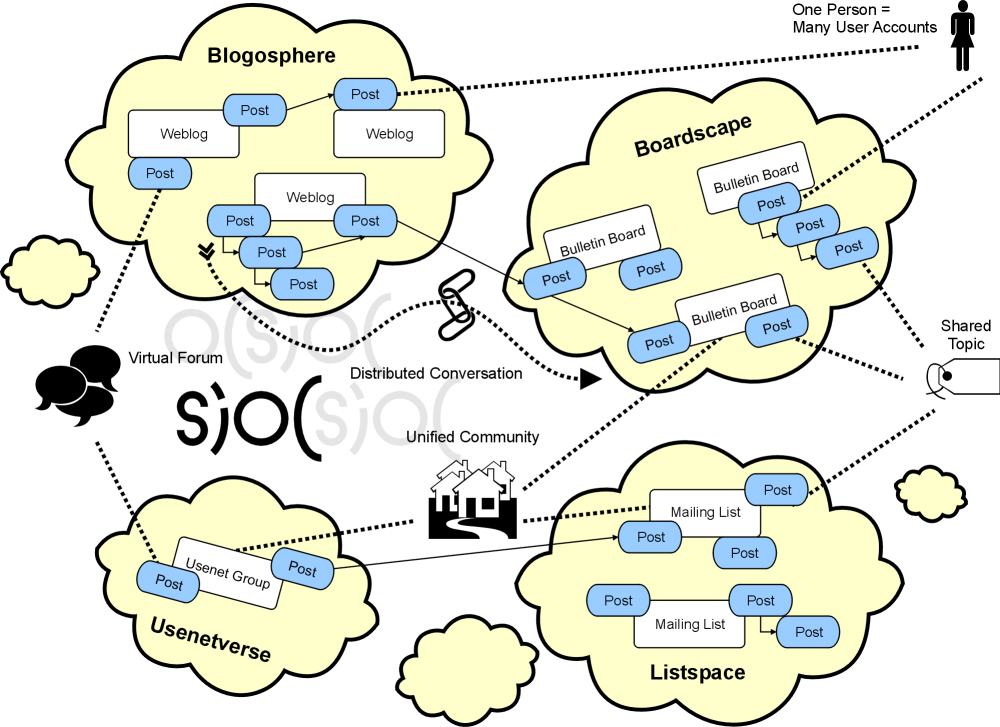
\includegraphics[width=12cm]{images/sioc-clouds.png}
	\caption{Conexiones de SIOC}
	\label{fig:siocCloud}
\end{figure}

Como se comenta en la sección~\ref{sec:ont:0.2}, SIOC modela una clase denominada
\texttt{sioc:Forum} que define un esquema (casi) completo para describir
semánticamente listas de correo. Además, tal y como se muestra en la 
figura~\ref{fig:sioc+foaf+skos}\footnote{Imagen original de John Breslin en 
\url{http://sioc-project.org/node/158}}, utiliza con gran acierto otras ontologías 
relacionadas.

\begin{figure}[H]
	\centering
	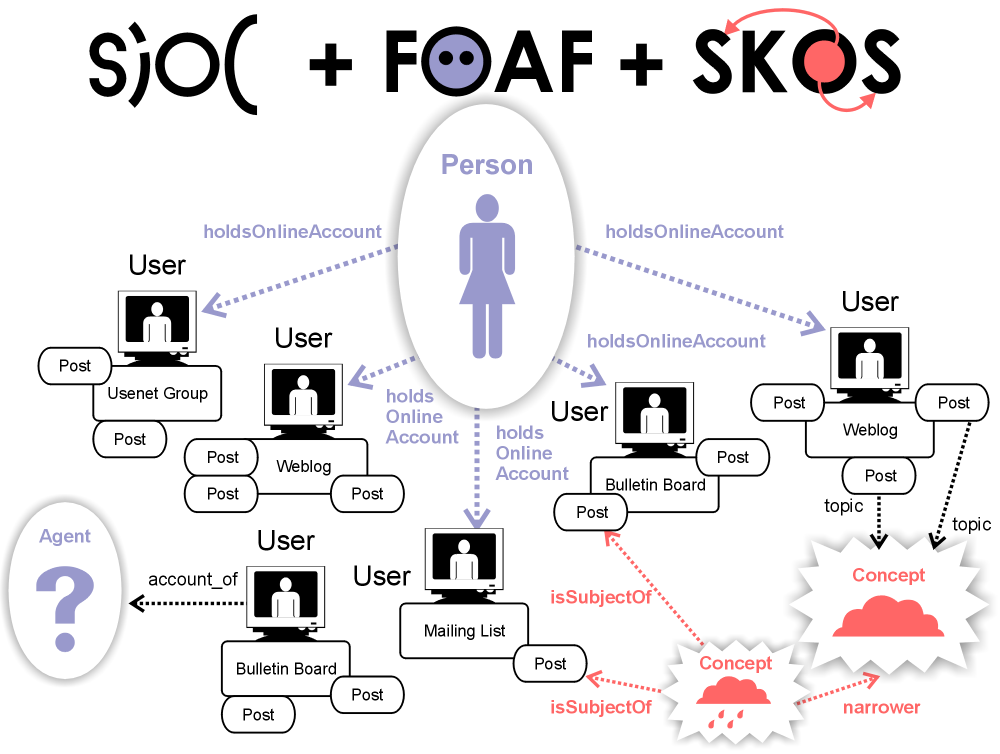
\includegraphics[width=9cm]{images/sioc-foaf-skos.png}
	\caption{Algunas ontologias relacionadas con SIOC}
	\label{fig:sioc+foaf+skos}
\end{figure}

Por tanto SIOC fue la opción escogida sobre la que construir SWAML. Utilizar SIOC
implicitamente significa que se usarán otras ontologías como FOAF y Dublin Core,
de las que hablará próximamente más en profundidad.


\subsection{Exportación de la información}

Una vez determinado que SIOC sería la ontología a utilizar, es necesario evaluar
las distintas posibilidades para la parte software más grande del proyecto.

Existe un gran abanico de software que exporta listas de correo. Pero todos
ellos (Pipermail\footnote{\url{http://www.amk.ca/python/unmaintained/pipermail.html}},
Hypermail\footnote{\url{http://www.hypermail-project.org/}}, etc) exportan únicamente
a formatos formatos orientados a la presentación final (principalmente HTML). 
Técnicamente parece complicado adaptar alguno: no disponen de API's, código bastante
viejo sin mantener, etc.

Respecto a software que realice la misma función pero a un formato semánticamente 
rico, apenas se encontraron dos alternativas:

\begin{itemize}
  \item El ya mencionado XMTP\footnote{\url{http://www.openhealth.org/xmtp/}}, un
	proyecto desarrollado en Java y abandonado desde 2001.
  \item aboutMsg.py\footnote{\url{http://www.w3.org/2000/04/maillog2rdf/aboutMsg.py}}, un
	proyecto desarrolado en Python por Dan Connolly\footnote{\url{http://www.w3.org/People/Connolly/}}
	que exporta a RDF/XML mensajes de correo electrónico sobre el esquema 
	swap/pim/email\footnote{\url{http://www.w3.org/2000/10/swap/pim/email}}
	antes mencionado.
  \item RDFizers\footnote{\url{http://simile.mit.edu/RDFizers/}} tiene un subproyecto
	llamado email2rdf\footnote{\url{http://simile.mit.edu/repository/RDFizers/email2rdf/}}
	que mediante una serie de scripts en Python exporta un mbox a RDF.
\end{itemize}

Los tres proyectos, al ser públicos, pudieron descargarse para ser estudiados más a fondo. Después
de varias pruebas se llegó a una conclusión: ninguno cubria mínimamente los requisitos (tantos 
funcionales como no funcionales) planteados. Por tanto, y después de analizar el alcanze del
proyecto, se concluyó que lo más sensato sería afrontar desde cero un nuevo desarrollo, sin las 
restricciones de diseño impuestas de utilizar código heredado de alguno de esos proyectos 
mencionados.

\begin{figure}[H]
	\centering
	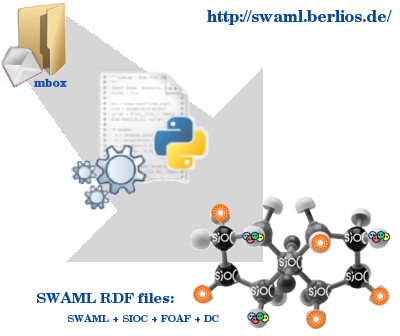
\includegraphics[width=9cm]{images/swaml-process.png}
	\caption{Futuro proceso software de SWAML}
	\label{fig:swamlProcess}
\end{figure}


\subsection{Consumición de la información}

SIOC aún no dispone de demasiadas implementaciones\footnote{\url{http://esw.w3.org/topic/SIOC/Implementations}},
y la mayor parte se concentran en la fase de exportación de datos de otros
tipos de foros (principalmente blogs). 

Respecto a la fase de consumir los datos el catálogo de aplicaciones es aún 
menor; únicamente existe dos aplicación especializadas en \emph{leer} de datos 
en SIOC:

\begin{itemize}
  \item SIOC Browser\footnote{\url{http://sioc-project.org/browser}} es un 
	navegador de información en RDF en general y SIOC en particular. 
	Esta escrito en Python como CGI para proveer una interfaz en HTML.
  \item SIOC live query\footnote{\url{http://b4mad.net/datenbrei/archives/2006/06/05/sioc-live-query/}},
	escrito en PHP, es una interfaz HTML para realizar consultas
	contra ficheros SIOC (predefinidos y no personalizables).
\end{itemize}

Ninguno hace operaciones más allá de realizar simples consultas a un único fichero 
SIOC. Por ello, y siempre que no alargue mucho los plazos del proyecto, puede ser 
interesante abordar el desarrollo de una aplicación que explote más profundamente
los datos exportados.
